\documentclass{amsart}

\usepackage{amssymb, amsfonts, hyperref, graphicx, bbm}
\usepackage{enumerate}

\newtheorem{thm}{Theorem}[section]
\newtheorem{cor}[thm]{Corollary}
\newtheorem{prop}[thm]{Proposition}
\newtheorem{lem}[thm]{Lemma}

\theoremstyle{definition}
\newtheorem{defn}[thm]{Definition}
\newtheorem{defns}[thm]{Definitions}
\newtheorem{con}[thm]{Construction}
\newtheorem{exmp}[thm]{Example}
\newtheorem{exmps}[thm]{Examples}
\newtheorem{notn}[thm]{Notation}
\newtheorem{notns}[thm]{Notations}
\newtheorem{addm}[thm]{Addendum}
\newtheorem{exer}[thm]{Exercise}

\theoremstyle{remark}
\newtheorem{rem}[thm]{Remark}
\newtheorem{rems}[thm]{Remarks}
\newtheorem{warn}[thm]{Warning}
\newtheorem{sch}[thm]{Scholium}

\bibliographystyle{plain}

\graphicspath{ {../figures/} }

%--------Meta Data: Fill in your info------
\title{Optimizing Multistage Portfolio Returns with Risk Constraints}

\author{Kurt Ehlert}

\date{\today}

\begin{document}

\begin{abstract}

TODO here goes the abstract

\end{abstract}

\maketitle

\tableofcontents

\section{Modeling Stocks with Geometric Brownian Motion}
Stochastic differential equations (SDEs) are commonly used to model stock prices over time. In particular,
geometric Brownian motion (GBM) is often used.\cite{hull} In this paper, we will use GBM with constant coefficients to model stock prices over time. The SDE for GBM is
\begin{equation}\label{eq:GBM_SDE}
dX_t = \mu X_t dt + \sigma X_t dB_t
\end{equation}
where $\mu$ and $\sigma$ are respectively the drift and volatility parameters, and $B_t$ is Brownian motion at time $t$. We call $X_t$ GBM, and see figure \ref{fig:mesh1} for some example GBM paths.

\begin{figure}
\centering
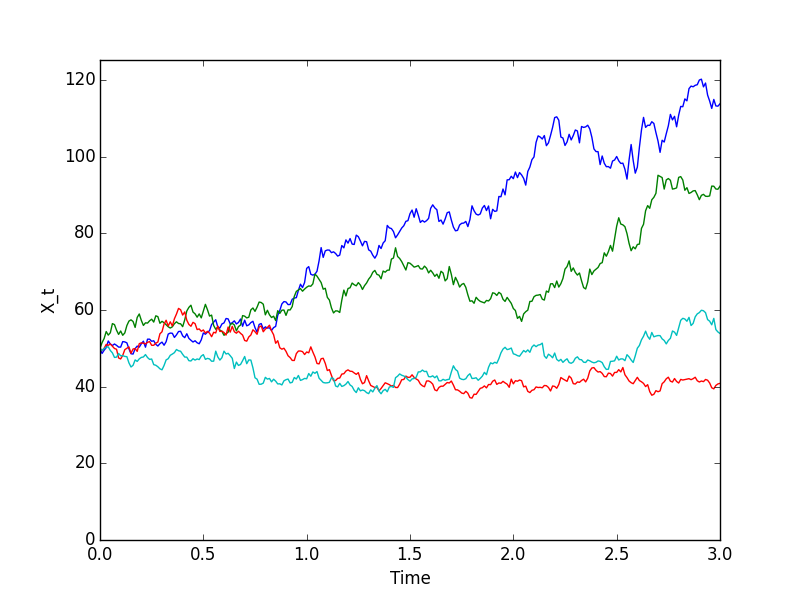
\includegraphics[scale=0.5]{geometric_bm.png}
\caption{Paths of geometric Brownian motion generated by the Euler-Maruyama method. Code can be found at TODO. $X_0 = 50, \mu=0.1, \sigma=0.2$.}
\label{fig:mesh1}
\end{figure}

\subsection{1-D Geometric Brownian Motion}
We can solve \eqref{eq:GBM_SDE} by using an integrating factor $Z_t$ \cite[p. 235]{timo}:
\begin{equation*}
Z_t = \exp\left(-\mu t -\sigma B_t + \sigma^2 t/2 \right)
\end{equation*}
For most of the following calculations, we will drop the subscript $t$. By It\^o's lemma we know that
\begin{equation}\label{eq:GBM_SDE_PROD}
d(XZ) = X dZ + Z dX + d[X,Z]
\end{equation}
where $[\cdot,\cdot]$ denotes quadratic covariation. The goal is to substitute in expressions for each of the variables on the right-hand side of the above expression. It\^o's lemma gives us $dZ$
\begin{equation*}
dZ = Z \left[\left(-u + \sigma^2\right) dt - \sigma dB\right]
\end{equation*}
Now we need to calculate the quadratic covariation of $X$ and $Z$,
\begin{align*}
\begin{split}
d[X,Z]_t &= d\left[\int_0^t \mu X_s ds + \int_0^t \sigma X_s dB_s,  \int_0^t (-\mu +\sigma^2) Z_s ds - \int_0^t \sigma Z_s dB_s \right]_t\\
&= d\left[\int_0^t \sigma X_s dB_s,  - \int_0^t \sigma Z_s dB_s \right]_t\\
&= -\sigma ^2 \frac{d}{dt}\int_0^t X_s Z_s ds\\
&= -\sigma^2 X_t Z_t dt
\end{split}
\end{align*}
Thus \eqref{eq:GBM_SDE_PROD} becomes
\begin{align*}
d(XZ) &= Z(\mu X dt + \sigma X dB) + XZ\left[\left(-\mu + \sigma^2 \right)dt -\sigma dB \right] - \sigma^2 X Z dt
&= 0
\end{align*}
Therefore $X_t Z_t = X_0 Z_0 = X_0$, which implies that
\begin{equation}\label{eq:GBM_soln}
X_t =  X_0 Z_t^{-1} = X_0 \exp\left[(\mu - \sigma^2/2) t + \sigma B_t\right]
\end{equation}
Then use It\^o's lemma to check that \eqref{eq:GBM_soln} solves \eqref{eq:GBM_SDE}. It is clear that $\log(X)$ is normally distributed, and
\begin{align*}
\mathbb{E}[\log X ] &= (\mu - \sigma^2/2)t\\
\text{Var}(\log X ) &= \sigma^2 t
\end{align*} 
Thus $X_t$ has a log-normal distribution, and
\begin{align*}
\mathbb{E} X&= X_0 e^\mu\\
\text{Var}X &= X_0^2 e^{2\mu t}(e^{\sigma^2 t} - 1)
\end{align*}

\subsection{Correlated d-Dimensional Geometric Brownian Motion}
If the Brownian motions driving each SDE are all independent, then the solution is just the d-dimensional version of \eqref{eq:GBM_soln}. The much more interesting case is when there is a positive correlation between the different dimensions. In other words, we want to find and solve the SDE where $X(t)$ is d-dimensional GBM and $\text{Corr}(X_i(t), X_j(t)) = \rho_{ij}$. This would allow us to model correlated stock prices.

\section{Optimizing a Portfolio}
Assume that there are $n$ stocks we can invest in, and also one risk-free asset that gives a constant rate of return $r$. We will model the path of all the stock prices as $n$ independent geometric Brownian motions. The average rate of return (also known as drift) and the volatility of each stock can vary.

If we simply want to maximize the expected return, then we should put all of our money into the asset with the highest expected return. However, that is not a very sensible approach, because it does not take into account our risk tolerance. The goal of this section is to present two approaches for balancing the expected return and the risk. The first approach is the one used by Markowitz, where we will maximize the return subject to a constraint on the variance of the return. The second method is to maximize the return subject to a constraint on the conditional value-at-risk (CV@R).

\subsection{Markowitz's approach}
\subsubsection{Portfolio Optimization Problem Description}
Suppose that we have $W$ dollars to invest, and we want to maximize the expected return after time $T$. However, we also want to keep the variance of the return below a specified level. There are $n$ stocks to invest in. Let $X_i(t)$ be the price of stock $i$ at time $t$. As mentioned earlier, we model the stock prices as independent paths of geometric Brownian motion. Therefore $X_i(t)$ is log-normally distributed, and
\begin{align*}
\mathbb{E} X_i(t) &= X_i(0)e^{\mu_i t}\\
\text{Var} X_i(t) &= X_i(0)^2e^{2\mu_i t}\left(e^{\sigma_i^2 t} -1\right)
\end{align*}
Let $R_i$ be the random return of stock $i$.
\begin{equation*}
R_i = \frac{X_i(t)}{X_i(0)} \implies \log R_i = (\mu_i - \sigma_i^2 / 2) t + \sigma dB_t
\end{equation*}
Therefore the return $R_i$ is also log-normally distributed, with
\begin{align*}
\mathbb{E}R_i &= e^{\mu_i t}\\
\text{Var}R_i &= e^{2\mu_i t}\left(e^{\sigma_i^2 t} -1\right)
\end{align*}

There is also a risk-free asset with a constant rate of return $r$. Let $x_i$ be the amount of capital allocated to stock $i$, and $x_r$ be the amount of capital invested in the risk-free asset. Let $C(x, R_i)$ be the amount of capital we have at time $t$. Then
\begin{equation*}
C(x, R_i) = r x_r + \sum_{i=1}^n R_i x_i 
\end{equation*}
and let $C$ be the capital we have at $t=0$.
Let $\Sigma$ be the $n\times n$ covariance matrix of the stocks. Then
\begin{align*}
\text{Var}[ C(x,R_i)] = x^T \Sigma x
\end{align*}
Thus the problem we want to solve is
\begin{equation}\label{eq:markowitz}
\max_{x,x_r\ge 0} \mathbb{E}C(x, R_i) = r x_r + \sum_{i=1}^n x_i e^{\mu_i t}, x^T \Sigma x \le v, x^T \mathbbm{1} + x_r \le C
\end{equation}
where $x$ is the vector of the stock allocations and $\mathbbm{1}$ is the column vector of all ones.
We can actually solve the above problem with Lagrange multipliers.

\subsubsection{Solving the Markowitz Portfolio Optimization Problem}
We do not prove that that Lagrange multiplier are applicable to this optimization problem, but they do work. Let $\bar{\mu}_i = e^{\mu_i t},$ and $\bar{r} = e^{rt}$.

\begin{thm}
The solution to the portfolio optimization problem \eqref{eq:markowitz} is
\begin{align*}
x &= \frac{\sqrt{v} \Sigma^{-1} (\bar{\mu} - \bar{r}\mathbbm{1})}{\sqrt{(\bar{\mu} - \bar{r}\mathbbm{1}) \Sigma^{-1} (\bar{\mu} - \bar{r}\mathbbm{1})}}\\
x_r &= C - x^T \mathbbm{1}
\end{align*}
\end{thm}
\begin{proof}
The Lagrange function corresponding to \eqref{eq:markowitz} is
\begin{equation*}
L(x,x_r,\lambda) = \bar{r} x_r + \bar{\mu}^T x + \lambda_1(x^T \Sigma x - v) + \lambda_2(x^T \mathbbm{1} + x_r - C)
\end{equation*}

The derivatives of $L$ are
\begin{align*}
\nabla_x L &= \bar{\mu} + 2\lambda_1\Sigma x + \lambda_2 \mathbbm{1}\\
\frac{\partial L}{\partial x_r} &= \bar{r}+\lambda_2\\
\frac{\partial L}{\partial \lambda_1} &= x^T \Sigma x - v\\
\frac{\partial L}{\partial \lambda_2} &= x^T \mathbbm{1} + x_r - C
\end{align*}

Setting $\nabla_x L$ and solving for $x$ implies that
\begin{equation}\label{eq:x_in_terms_lambda}
x = -\frac{1}{2\lambda_1} \Sigma^{-1}(\bar{\mu} - \bar{r}\mathbbm{1})
\end{equation}
Now if we set $\frac{\partial L}{\partial \lambda_1} = 0$, we have $x^T\Sigma x = v$. Substituting the above expression for $x$ into $x^T\Sigma x = v$ gives
\begin{equation*}
\frac{1}{4\lambda_1^2} (\bar{\mu}-\bar{r}\mathbbm{1})^T\Sigma^{-1} (\bar{\mu}-\bar{r}\mathbbm{1}) = v
\end{equation*}
Solving for $\lambda_1$ leads to
\begin{equation*}
\lambda_1 = \pm \frac{1}{2\sqrt{v}} \sqrt{(\bar{\mu}-\bar{r}\mathbbm{1})^T\Sigma^{-1} (\bar{\mu}-\bar{r}\mathbbm{1})}
\end{equation*}
Substituting that expression for $\lambda_1$ back into \eqref{eq:x_in_terms_lambda} gives us the solution for $x$. Now set $\frac{\partial L}{\partial \lambda_1} = 0$ (i.e. use the capital constraint) to get the solution for $x_r$.
\end{proof}

There is Python code in the appendix that tests the Lagrange multiplier solution (TODO). It compares the Lagrange solution to a solution obtained by Gurobi. For the example parameters, the Lagrange solution is actually slightly better than Gurobi's. The output is in the appendix (TODO).

\subsection{V@R, CV@R}


\subsection{multistage}

\subsection*{Acknowledgments}  I downloaded and then modified the \LaTeX template at \url{www.math.uchicago.edu/~may/VIGRE/VIGRE2011/TEMPLATE.tex}

\bibliography{719_project}
\bibliographystyle{ieeetr}

\end{document}

